\documentclass{standalone}
\usepackage{tikz}
\usetikzlibrary{patterns, positioning}
\usepackage[sfdefault]{ClearSans} %% option 'sfdefault' activates Clear Sans as the default text font
\usepackage[T1]{fontenc}

\begin{document}
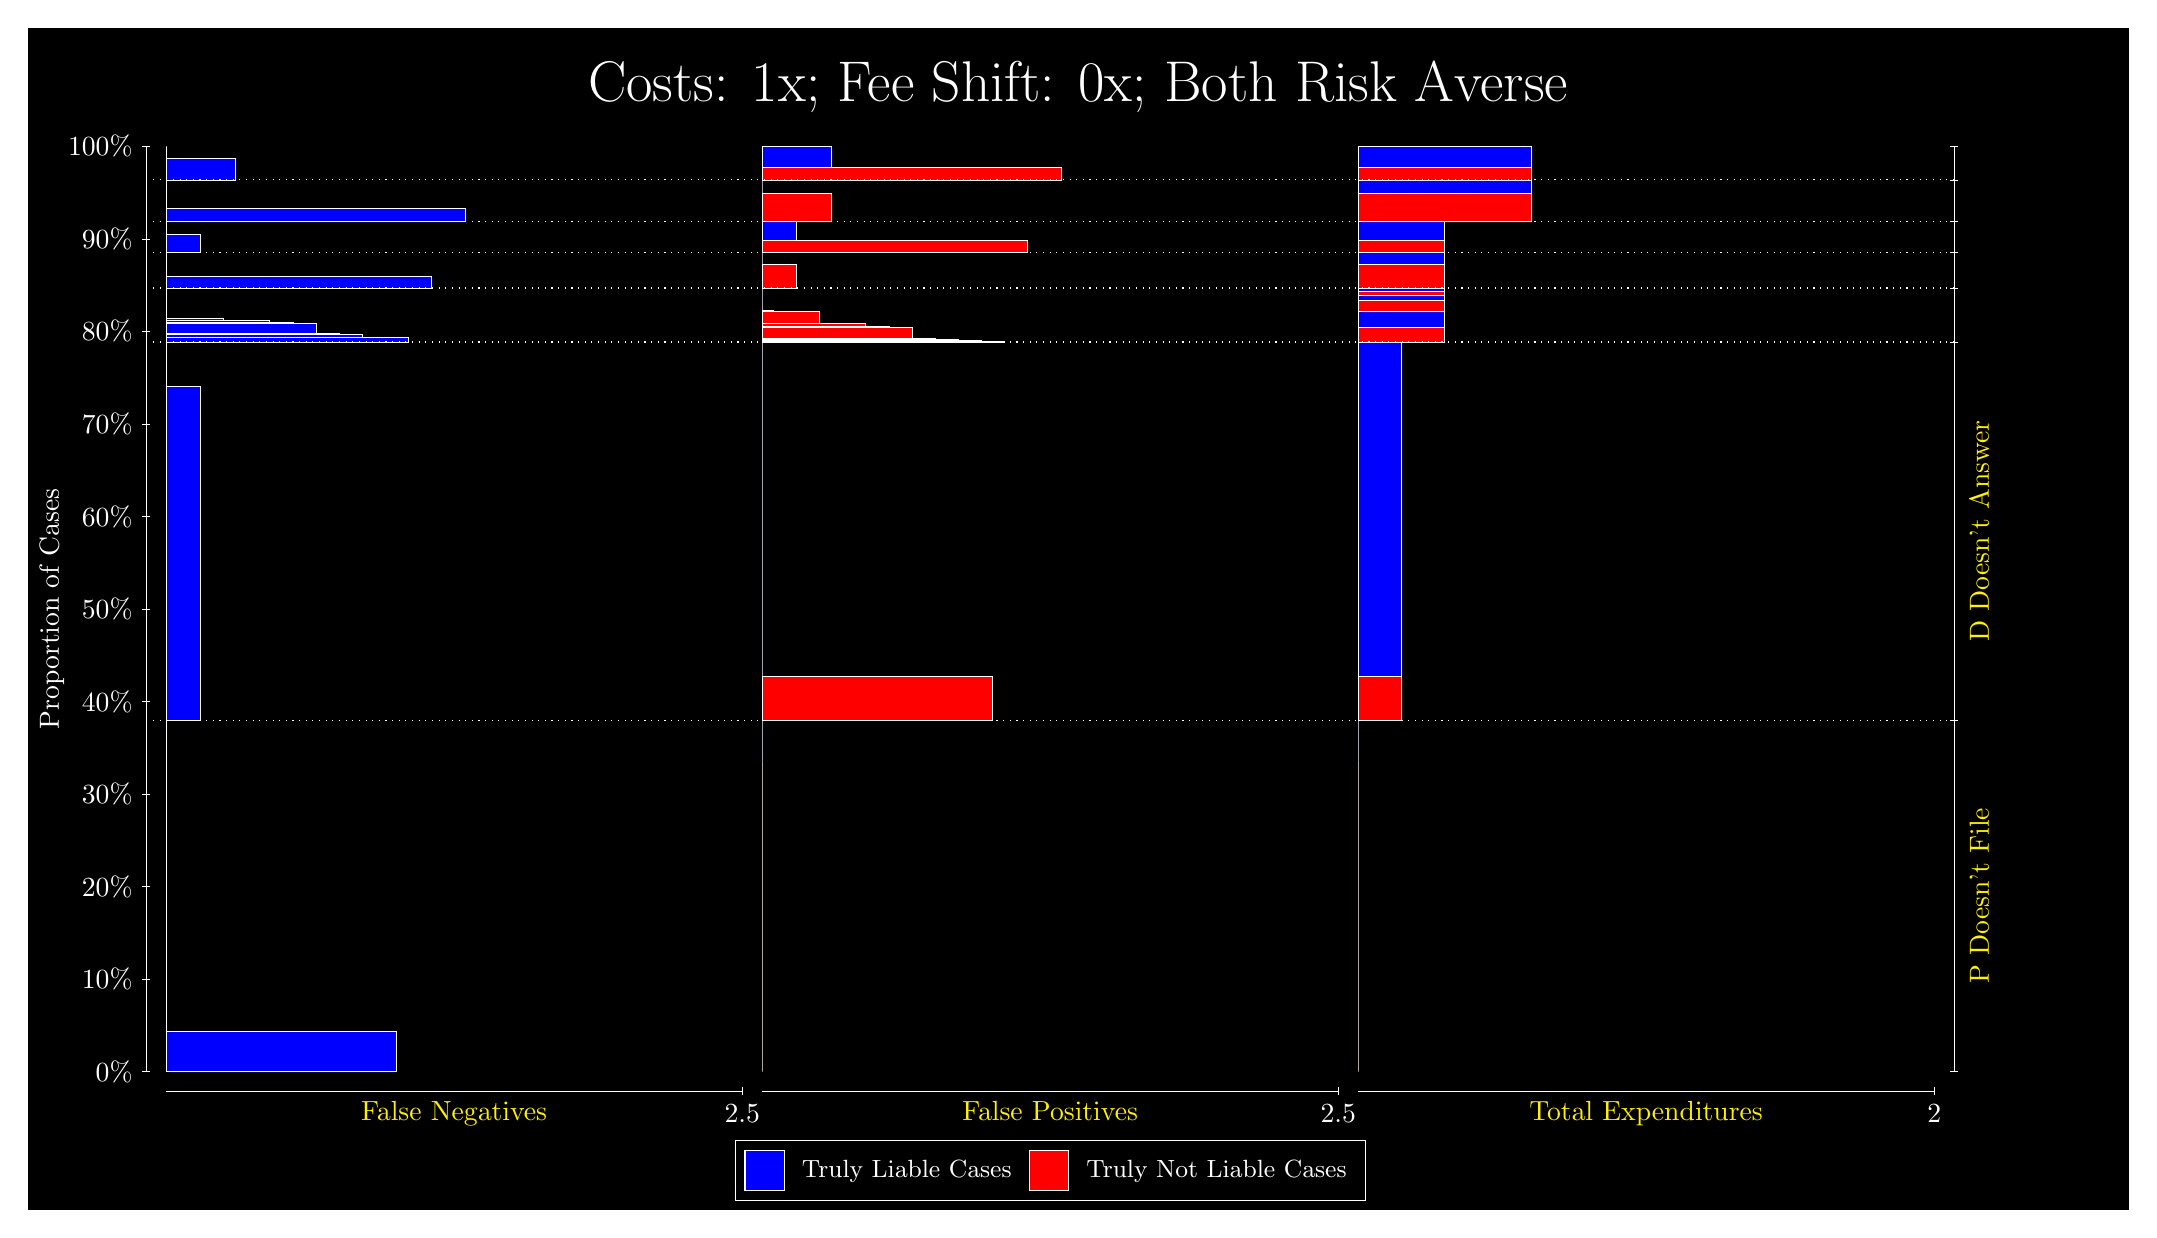
\begin{tikzpicture}
\draw[fill=black] (0,0) rectangle (26.667,15);
\draw[text=white] (0,13.5) rectangle (26.667,15) node[midway] {\huge Costs: 1x; Fee Shift: 0x; Both Risk Averse};
\draw[white, very thin] (1.5,1.75) -- (1.5,13.5);
\node[rotate=90, text=white, anchor=center] at (0.3, 7.625) {Proportion of Cases};
\draw[white, very thin] (1.45,1.75) -- (1.55,1.75);
\node[text=white, anchor=east] at (1.45, 1.75) {0\%};
\draw[white, very thin] (1.45,2.925) -- (1.55,2.925);
\node[text=white, anchor=east] at (1.45, 2.925) {10\%};
\draw[white, very thin] (1.45,4.1) -- (1.55,4.1);
\node[text=white, anchor=east] at (1.45, 4.1) {20\%};
\draw[white, very thin] (1.45,5.275) -- (1.55,5.275);
\node[text=white, anchor=east] at (1.45, 5.275) {30\%};
\draw[white, very thin] (1.45,6.45) -- (1.55,6.45);
\node[text=white, anchor=east] at (1.45, 6.45) {40\%};
\draw[white, very thin] (1.45,7.625) -- (1.55,7.625);
\node[text=white, anchor=east] at (1.45, 7.625) {50\%};
\draw[white, very thin] (1.45,8.8) -- (1.55,8.8);
\node[text=white, anchor=east] at (1.45, 8.8) {60\%};
\draw[white, very thin] (1.45,9.975) -- (1.55,9.975);
\node[text=white, anchor=east] at (1.45, 9.975) {70\%};
\draw[white, very thin] (1.45,11.15) -- (1.55,11.15);
\node[text=white, anchor=east] at (1.45, 11.15) {80\%};
\draw[white, very thin] (1.45,12.325) -- (1.55,12.325);
\node[text=white, anchor=east] at (1.45, 12.325) {90\%};
\draw[white, very thin] (1.45,13.5) -- (1.55,13.5);
\node[text=white, anchor=east] at (1.45, 13.5) {100\%};

\draw[white, very thin] (24.457,1.75) -- (24.457,13.5);
\draw[white, very thin] (24.407,1.75) -- (24.507,1.75);
\node[anchor=west] at (24.407, 1.75) {};
\draw[white, very thin] (24.407,6.2129) -- (24.507,6.2129);
\node[anchor=west] at (24.407, 6.2129) {};
\draw[white, very thin] (24.407,11.015) -- (24.507,11.015);
\node[anchor=west] at (24.407, 11.015) {};
\draw[white, very thin] (24.407,11.701) -- (24.507,11.701);
\node[anchor=west] at (24.407, 11.701) {};
\draw[white, very thin] (24.407,12.15) -- (24.507,12.15);
\node[anchor=west] at (24.407, 12.15) {};
\draw[white, very thin] (24.407,12.542) -- (24.507,12.542);
\node[anchor=west] at (24.407, 12.542) {};
\draw[white, very thin] (24.407,13.074) -- (24.507,13.074);
\node[anchor=west] at (24.407, 13.074) {};
\draw[white, very thin] (24.407,13.5) -- (24.507,13.5);
\node[anchor=west] at (24.407, 13.5) {};

\draw[white, very thin, fill=blue] (1.75,1.75) rectangle (4.6775,2.2614);
\draw[white, very thin, fill=red] (1.75,2.2614) rectangle (1.75,6.2129);
\draw[white, very thin, fill=blue] (1.75,6.2129) rectangle (2.1891,10.454);
\draw[white, very thin, fill=red] (1.75,10.454) rectangle (1.75,11.015);
\draw[white, very thin, fill=blue] (1.75,11.015) rectangle (4.8239,11.073);
\draw[white, very thin, fill=blue] (1.75,11.073) rectangle (4.5312,11.078);
\draw[white, very thin, fill=blue] (1.75,11.078) rectangle (4.2384,11.114);
\draw[white, very thin, fill=blue] (1.75,11.114) rectangle (3.9457,11.125);
\draw[white, very thin, fill=blue] (1.75,11.125) rectangle (3.6529,11.251);
\draw[white, very thin, fill=blue] (1.75,11.251) rectangle (3.3602,11.269);
\draw[white, very thin, fill=blue] (1.75,11.269) rectangle (3.0674,11.288);
\draw[white, very thin, fill=blue] (1.75,11.288) rectangle (2.7746,11.292);
\draw[white, very thin, fill=blue] (1.75,11.292) rectangle (2.4819,11.312);
\draw[white, very thin, fill=red] (1.75,11.312) rectangle (1.75,11.701);
\draw[white, very thin, fill=blue] (1.75,11.701) rectangle (5.1167,11.852);
\draw[white, very thin, fill=red] (1.75,11.852) rectangle (1.75,12.15);
\draw[white, very thin, fill=blue] (1.75,12.15) rectangle (2.1891,12.386);
\draw[white, very thin, fill=red] (1.75,12.386) rectangle (1.75,12.542);
\draw[white, very thin, fill=blue] (1.75,12.542) rectangle (5.5558,12.712);
\draw[white, very thin, fill=red] (1.75,12.712) rectangle (1.75,13.074);
\draw[white, very thin, fill=blue] (1.75,13.074) rectangle (2.6283,13.343);
\draw[white, very thin, fill=red] (1.75,13.343) rectangle (1.75,13.5);
\draw[white, very thin, fill=red] (9.3189,1.75) rectangle (9.3189,5.7015);
\draw[white, very thin, fill=blue] (9.3189,5.7015) rectangle (9.3189,6.2129);
\draw[white, very thin, fill=red] (9.3189,6.2129) rectangle (12.246,6.7731);
\draw[white, very thin, fill=blue] (9.3189,6.7731) rectangle (9.3189,11.015);
\draw[white, very thin, fill=red] (9.3189,11.015) rectangle (12.393,11.026);
\draw[white, very thin, fill=red] (9.3189,11.026) rectangle (12.1,11.031);
\draw[white, very thin, fill=red] (9.3189,11.031) rectangle (11.807,11.05);
\draw[white, very thin, fill=red] (9.3189,11.05) rectangle (11.515,11.068);
\draw[white, very thin, fill=red] (9.3189,11.068) rectangle (11.222,11.198);
\draw[white, very thin, fill=red] (9.3189,11.198) rectangle (10.929,11.206);
\draw[white, very thin, fill=red] (9.3189,11.206) rectangle (10.929,11.211);
\draw[white, very thin, fill=red] (9.3189,11.211) rectangle (10.636,11.251);
\draw[white, very thin, fill=red] (9.3189,11.251) rectangle (10.344,11.256);
\draw[white, very thin, fill=red] (9.3189,11.256) rectangle (10.051,11.404);
\draw[white, very thin, fill=blue] (9.3189,11.404) rectangle (9.4652,11.424);
\draw[white, very thin, fill=blue] (9.3189,11.424) rectangle (9.3189,11.701);
\draw[white, very thin, fill=red] (9.3189,11.701) rectangle (9.758,12);
\draw[white, very thin, fill=blue] (9.3189,12) rectangle (9.3189,12.15);
\draw[white, very thin, fill=red] (9.3189,12.15) rectangle (12.686,12.306);
\draw[white, very thin, fill=blue] (9.3189,12.306) rectangle (9.758,12.542);
\draw[white, very thin, fill=red] (9.3189,12.542) rectangle (10.197,12.904);
\draw[white, very thin, fill=blue] (9.3189,12.904) rectangle (9.3189,13.074);
\draw[white, very thin, fill=red] (9.3189,13.074) rectangle (13.125,13.231);
\draw[white, very thin, fill=blue] (9.3189,13.231) rectangle (10.197,13.5);
\draw[white, very thin, fill=red] (16.888,1.75) rectangle (16.888,5.7015);
\draw[white, very thin, fill=blue] (16.888,5.7015) rectangle (16.888,6.2129);
\draw[white, very thin, fill=red] (16.888,6.2129) rectangle (17.437,6.7731);
\draw[white, very thin, fill=blue] (16.888,6.7731) rectangle (17.437,11.015);
\draw[white, very thin, fill=red] (16.888,11.015) rectangle (17.986,11.206);
\draw[white, very thin, fill=blue] (16.888,11.206) rectangle (17.986,11.4);
\draw[white, very thin, fill=red] (16.888,11.4) rectangle (17.986,11.547);
\draw[white, very thin, fill=blue] (16.888,11.547) rectangle (17.986,11.606);
\draw[white, very thin, fill=red] (16.888,11.606) rectangle (17.986,11.656);
\draw[white, very thin, fill=blue] (16.888,11.656) rectangle (17.986,11.701);
\draw[white, very thin, fill=red] (16.888,11.701) rectangle (17.986,12);
\draw[white, very thin, fill=blue] (16.888,12) rectangle (17.986,12.15);
\draw[white, very thin, fill=red] (16.888,12.15) rectangle (17.986,12.306);
\draw[white, very thin, fill=blue] (16.888,12.306) rectangle (17.986,12.542);
\draw[white, very thin, fill=red] (16.888,12.542) rectangle (19.083,12.904);
\draw[white, very thin, fill=blue] (16.888,12.904) rectangle (19.083,13.074);
\draw[white, very thin, fill=red] (16.888,13.074) rectangle (19.083,13.231);
\draw[white, very thin, fill=blue] (16.888,13.231) rectangle (19.083,13.5);
\draw[white, dotted] (1.5,6.2129) -- (24.457,6.2129);
\draw[white, dotted] (1.5,11.015) -- (24.457,11.015);
\draw[white, dotted] (1.5,11.701) -- (24.457,11.701);
\draw[white, dotted] (1.5,12.15) -- (24.457,12.15);
\draw[white, dotted] (1.5,12.542) -- (24.457,12.542);
\draw[white, dotted] (1.5,13.074) -- (24.457,13.074);
\draw[white, very thin] (1.75,1.5) -- (9.0689,1.5);
\node[text=yellow, anchor=north] at (5.4094, 1.5) {False Negatives};
\draw[white, very thin] (9.0689,1.45) -- (9.0689,1.55);
\node[text=white, anchor=north] at (9.0689, 1.45) {2.5};

\draw[white, very thin] (9.3189,1.5) -- (16.638,1.5);
\node[text=yellow, anchor=north] at (12.978, 1.5) {False Positives};
\draw[white, very thin] (16.638,1.45) -- (16.638,1.55);
\node[text=white, anchor=north] at (16.638, 1.45) {2.5};

\draw[white, very thin] (16.888,1.5) -- (24.207,1.5);
\node[text=yellow, anchor=north] at (20.547, 1.5) {Total Expenditures};
\draw[white, very thin] (24.207,1.45) -- (24.207,1.55);
\node[text=white, anchor=north] at (24.207, 1.45) {2};

\node[text=yellow, centered, rotate=90] at (24.777, 3.9814) {P Doesn't File};
\node[text=yellow, centered, rotate=90] at (24.777, 8.6138) {D Doesn't Answer};






\draw (12.978300999999998,1.5) node[draw=none] (baseCoordinate) {};
\begin{scope}[align=center]
        \matrix[scale=0.5, draw=white, below=0.5cm of baseCoordinate, nodes={draw}, column sep=0.1cm]{
            \node[rectangle, draw, minimum width=0.5cm, minimum height=0.5cm, fill=blue] {}; &
            \node[draw=none, font=\small, text=white] (B) {Truly Liable Cases}; &
            \node[rectangle, draw, minimum width=0.5cm, minimum height=0.5cm, fill=red] {}; &
            \node[draw=none, font=\small, text=white] (B) {Truly Not Liable Cases}; \\
            };
\end{scope}

\end{tikzpicture}
\end{document}